\documentclass[notitlepage,letterpaper,12pt]{article} % para articulo

%\documentstyle[12pt,aas_macros]{article}

% Este es un comentario <- Los comentarios comienzan con % 
% todo lo que se escriba hasta el final de la linea será ignorado <- Este es otro comentario

%Encoding
\usepackage[utf8]{inputenc} % Acepta caracteres en castellano
\usepackage[T1]{fontenc} % Encoding de salida al pdf

%Lenguaje del documento
\usepackage[spanish]{babel} % silabea palabras castellanas <- Puedo poner comentarios para explicar de que va este comando en la misma línea
\usepackage{csquotes}


%Triunfó el mal
%\usepackage[normalem]{ulem}
%\useunder{\uline}{\ul}{}
\usepackage{aas_macros} %Para las citaciones de ADS Harvard
\usepackage[backend=bibtex8,sorting=none]{biblatex} %Para mejores citaciones
\providecommand{\e}[1]{\ensuremath{\times 10^{#1}}} %notación científica

\def\sen{\mathop{\mbox{\normalfont sen}}\nolimits} %La opción de usar sen en vez de sin con \sen

\usepackage{textcomp}
\usepackage{gensymb}



%Hipertexto
\usepackage[colorlinks=true,urlcolor=blue,linkcolor=blue]{hyperref} % navega por el doc: hipertexto y links

%Aquello de las urls
\usepackage{url} 

%simbolos matemáticos
\usepackage{amsmath}
\usepackage{amsfonts}
\usepackage{amssymb}
\usepackage{physics} 

% permite insertar gráficos, imágenes y figuras, en pdf o en eps
\usepackage{graphicx}
\usepackage{epstopdf}
\usepackage{multirow}
\usepackage[export]{adjustbox}
% geometría del documento, encabezados y pies de páginas, márgenes
\usepackage{quotmark} %Uso consistente con la RAE de comillas
\usepackage{geometry}     
\geometry{letterpaper}       % ... o a4paper o a5paper o ... 
\usepackage{fancyhdr} % encabezados y pies de pg
\pagestyle{fancy}
\chead{\bfseries {}}
\lhead{} % si se omite coloca el nombre de la seccion
%\rhead{fecha del doc}
\lfoot{\it Avance del proyecto.}
\cfoot{ }
\rfoot{Universidad de los Andes}
%\rfoot{\thepage}
%margenes
\voffset = -0.25in
\textheight = 8.0in
\textwidth = 6.5in
\oddsidemargin = 0.in
\headheight = 20pt
\headwidth = 6.5in
\renewcommand{\headrulewidth}{0.5pt}
\renewcommand{\footrulewidth}{0,5pt}

\addbibresource{bibtex.bib}


\begin{document}
\title{Medición de la velocidad de rotación de estrellas de alta temperatura (tipo O, B y A)}
\author{
\textbf{Javier Alejandro Acevedo Barroso\thanks{e-mail: \texttt{ja.acevedo12@uniandes.edu.co}}}\vspace{2mm} \\
Directores:\\
\textbf{Alejandro García Ph.D}\\
\textbf{Beatriz Sabogal Ph.D}
} % Hasta aquí llega el bloque "author" (son dos autores por informe, orden alfabético)

%\date{Versión $\alpha \beta$ fecha del documento }
\maketitle %Genera el título del documento


%Resumen
\vspace{-6mm}
\begin{abstract}
%TODO:abstract
En este proyecto se medirá la velocidad de rotación de al menos una estrella de tipo espectral O, B o A comparando el FWHM de las líneas de Helio y Magnesio de la estrella con lineas de emisión simuladas a diferentes velocidades de rotación, o con una escala definida para ese tipo espectral de estrella. En este trabajo se responderá a las preguntas: ¿se puede medir la velocidad de rotación espectral de una estrella en el cielo de Bogotá con el equipamento del observatorio de la universidad (OAU)? ¿Cómo se compara la medición (incluyendo la incertidumbre) con los valores reportados en la literatura?
\end{abstract} 
%Introducción
\section{Introducción} 
Durante siglos, el estudio de las estrellas ha sido esencial para la humanidad, desde el desarrollo de calendarios, hasta la medición de distancias cosmológicas. En particular, el estudio de la \emph{velocidad de rotación} de una estrella respecto a su propio eje da información sobre su proceso de formación, su achatamiento en los polos y su edad. Por lo tanto, la medición de la velocidad de rotación de una estrella es una importante herramienta para un astrónomo profesional. Adicionalmente, al ser un técnica espectroscópica, está considerablemente menos afectada por la contaminación atmosférica de la ciudad y el mal cielo. El proyecto se realizará bajo la supervisión de los profesores Beatriz Sabogal y Alejandro García, la toma de datos, al ser en el observatorio de la universidad, será supervisada por María Batista. 
%Los experimentos que realizaremos serán en el laboratorio de física de Altas energías, estaremos bajo la supervisión del profesor Carlos Ávila y del encargado del laboratorio Gerardo Roque.

\subsection*{Objetivos}
El objetivo principal del proyecto es medir la velocidad rotacional de al menos una estrella de tipo O, B o A, y compararla con valores de la literatura reportados recientemente.
Este objetivo general está acompañado de tres de objetivos específicos: tomar espectros de estrellas tipo O,B o A usando el equipamiento del observatorio; obtener familiaridad con la técnica del cálculo de la velocidad de rotación a partir del FWHM; y obtener familiaridad con la operación del equipo del observatorio, en particular, el telescopio Meade LX200 y el espectrógrafo eShel.

Estos objetivos se plantearon teniendo en cuenta el mal cielo característico de Bogotá y las dificultades de observación predecibles para el semestre. De ser posible, se espera medir la velocidad de rotación de más de una estrella, o poder repetir la medición para la misma estrella.

\section{Marco Teórico}
\subsection*{Medición de la velocidad de rotación}
La medición de la velocidad de rotación es una técnica espectroscópica que se vale del efecto Doppler para medir la velocidad de rotación proyectada.

El efecto Doppler es el cambio de frecuencia en una onda cuando hay una velocidad relativa entre la fuente y el observador. En el caso de la rotación estelar, una sección de la estrella estará alejandose de la tierra, mientras que la otra se estará acercando. Ambos efectos juntos corresponden a un ensanchamiento de las líneas de emisión de la estrella.
La representación esquemática del fenómeno se puede apreciar en la figura \ref{doppler}.

\begin{figure}[h!]
  \centering
%   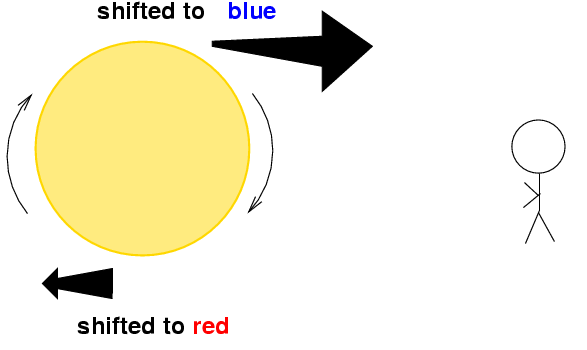
\includegraphics[scale= 0.5]{doppler.png}
  \caption{Efecto Doppler debido a la rotación de la estrella sobre su propio eje. Tomada de \cite{doppler} }
  \label{doppler}
\end{figure}

Sin embargo, dado que el eje de rotación de la estrella usualmente no es perpendicular a nuestro eje de observación, terminaremos observando una proyección de la verdadera velocidad de rotación. Sea $V$ la velocidad de rotación de una estrella en el ecuador. Si su eje rotación está inclinado respecto a la línea de visión de la tierra con un ángulo $i$, entonces la velocidad de rotación observada será:
\begin{equation}
v_{rot} = V \sen (i).
\end{equation}
Esta proyección se puede apreciar mejor en la figura \ref{proyeccion}. En este trabajo al hablar de velocidad de rotación, siempre se hablará de la velocidad rotacional proyectada ($v_{rot}$)

\begin{figure}[h!]
  \centering
%   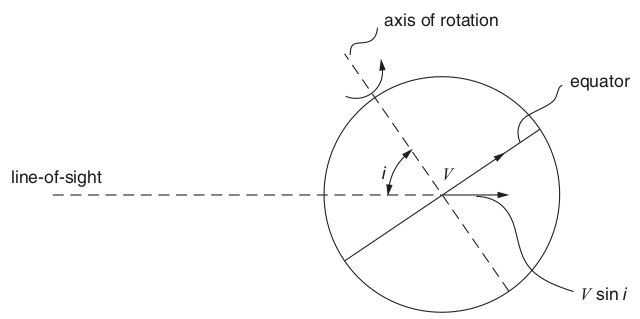
\includegraphics[scale= 0.5]{V_sin_i.png}
  \caption{Proyección de la velocidad de rotación ecuatorial $V$ debido a la inclinación entre el eje de rotación y la línea de visión de la tierra. Figura tomada de \cite{book:590711}.}
  \label{proyeccion}
\end{figure}

Por último, se considerarán dos maneras para relacionar el FWHM de las líneas medidas con la velocidad rotacional proyectada de la estrella:
\begin{itemize}
\item Simular las líneas de emisión de interés incluyendo diferentes posibles velocidades de rotación, al final, la velocidad reportada sería el mejor ajuste entre el modelo simulado y las líneas medidas. Las líneas simuladas deben incluir no solo el efecto Doppler de la rotación, sino también el oscurecimiento del limbo, el oscurecimiento gravitacional y el achatamiento de la estrella \cite{Slettebak} \cite{syntetic}. Para la simulación de la línea se utiliza códigos y algoritmos ya diseñados\cite{Przybilla}, el código final a utilizar dependerá del tipo de espectros que se logren captar antes del inicio de la temporada de lluvia.
\item El segundo método es usar una escala o catálogo que incluya el FWHM para diferentes estrellas junto a su correspondiente velocidad de rotación proyectada $v_e \sen i$ y tomar un espectro a alguna estrella de la escala similar al blanco de interés. Por ejemplo si se captura un espectro de Sirio (estrella tipo A1), se necesitaría de la escala una estrella en una posición cercana y también de tipo A1. Dada la relativa improbabilidad de encontrar tales estrellas, este método solo se utilizará en caso de efectivamente logra captar una estrella adecuada de la escala de calibración\cite{Slettebak}.
\end{itemize} 

%Montaje experimental
\section{Desarrollo experimental}
La realización del proyecto requiere la toma de espectros de al menos una estrella objetivo, una estrella de calibración de flujo, imágenes de calibración para las correcciónes de la cámara CCD, y si se puede, el espectro de una estrella de la escala. Se decidió estudiar estrellas de tipo O, B y A pues tienen líneas de Helio y Magnesio lo suficientemente fuertes para su análisis. Además ques son el tipo de estrella más luminoso y hay extensiva literatura sobre sus velocidad rotacionales \cite{syntetic} \cite{rotOfB} \cite{2004IAUS..224..109R}.

Dadas las adversas condiciones de observación que caracterizan a Bogotá\footnote{Contaminación lumínica, contaminación atmosférica, poco número de noches de observación al año, entre otros.} se decidió hacer una lista de estrellas blanco para cada bloque de 15 días. Esta lista se hizo usando el planetario virtual Stellarium, tomando las 8:00 pm como hora de observación.
Adicional a la lista de estrellas objetivo se debe tener estrellas de calibración para el flujo, para esto los observatorios profesionales fijan estándares espectrofotométricos \cite{flux4Hubble}. En este trabajo utilizaremos el estandar disponible más cercano a nuestra estrella objetivo, diferentes estrellas pueden tener diferentes estandares espectrofotométricos.

En principio con un espectro correctamente tomado por estrella objetivo sería suficiente para obtener la velocidad de rotación. Con el fin de ganar familiaridad con la técnica, y de obtener mejores mediciones, se tomará cuantos espectros sean posibles por estrella (en diferentes noches). Naturalmente, es necesario volver a tomar las imágenes de corrección de la cámara CCD (BIAS, FLATS y DARKS) y la estrella estandar estectrofotométrica por cada noche de observación.

Las predicciones meteorológicas señalan que hay temporada de lluvia desde mitad-finales de marzo hasta finales de mayo. Por lo anterior, se espera tomar la mayor cantidad de espectros en las semanas 5 a 8 del semestre. Sin embargo, la lista de estrellas objetivo incluye estrellas hasta la semana 14 del semestre, en caso de que se de una buena noche de observación. Los datos se tomarán entre 7 pm y 10 pm, de acuerdo al horario del observatorio. 

Para la toma de datos se utilizará el telescopio del observatorio Meade LX200 de 16 pulgadas y razón focal f/10. Para la toma de los espectros se utilizará el espectrógrafo eShel. El espectrógrafo es de tipo \enquote{echelle}, incluye su propia cámara CCD, una unidad de acople al telescopio y una colección pequeña de lámparas de calibración. El equipo a utilizar se puede apreciar en la figura \ref{equipo}




\begin{figure}[h!]
%   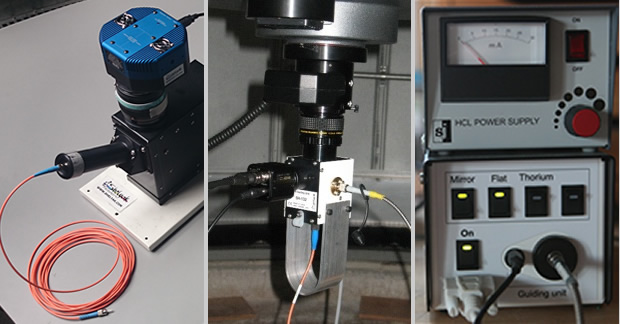
\includegraphics[scale= 0.6]{mosaico2.jpg} 
%   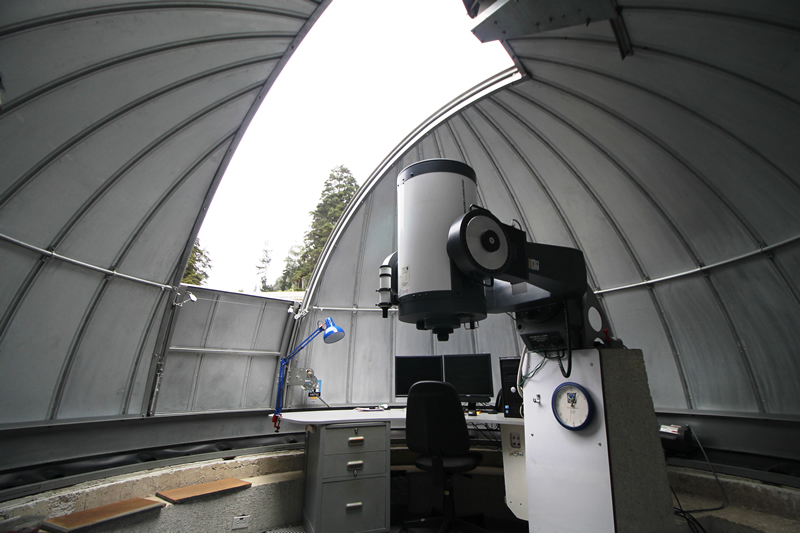
\includegraphics[scale = 0.28]{IMG_9512.JPG}
  \caption{Equipo a utilizar durante el proyecto. Izquierda: Espectrógrafo, unidad de acople al telescopio y lámpara de calibración. Derecha: observatorio de la universidad y el telescopio.}
  \label{equipo}
\end{figure}




% Puedo usar subsecciones para destacar un serie de párrafos que forman un marco común dentro de una sección:
%\subsection{Tablas}
%Las Tablas deben ser lo más autocontenidas posibles. Sus títulos y  leyendas deben ser suficiente para explicar su contenido. Las tablas deben ser referidas desde el texto (ver Tabla \ref{Tabla1}). Si no se hace referencia a una tabla en particular, ésta se considera inútil para el artículo y debe ser suprimida

Se espera tener al menos un espectro a más tardar la semana 8 del semestre. Una vez se tenga noches de observación exitosas, se procederá al análisis de los espectros que tomará desde la semana 8 hasta la 12. Se empezará a escribir el documento desde la semana 10 y continuará a un ritmo estable durante hasta la entrega final. En la semana 12 se presentará el avance con la velocidad de rotación proyectada de al menos una estrella. De la semana 12 hasta la entrega final del proyecto se procesará los nuevos espectros (si se logró continuar la toma de datos durante la temporada de lluvia) y se explorará mejores modelos o alternativas para el cálculo de la velocidad. En la semana 15 se entregará el documento final y se hará la presentación del poster. La revisión bibliográfica se realizó en la semana 5 y 6, y se realizará una última revisión en la semana 14 antes de la entrega final.




\section{Referencias}
\printbibliography[heading=none]
%Fin del documento
\end{document}


%Todo lo que escriba aquí será ignorado, aunque no fuera un comentario...
\begin{table}[h!]
\centering
\begin{tabular}{|l|l|l|}
\hline
2 cm   & 4 cm   & 8 cm   \\ \hline
175,77 & 129,77 & 88,77  \\ \hline
223,77 & 129,77 & 114,77 \\ \hline
219,77 & 134,77 & 77,77  \\ \hline
190,77 & 120,77 & 83,77  \\ \hline
\end{tabular}
\caption{Número de colisiones a diferentes distancias en cinco minutos.}
\label{tiempoFijo}
\end{table}


\begin{figure}[h]
  \centering
   \includegraphics[scale= 0.8]{jairos.png}
  \caption{Gráfica del periodo de la pulsación para diferentes razones entre las frecuencias naturales utilizando una pesa de 200g. Es de resaltar que el pico no está centrado en 1 pero está bastante cerca. Esto probablemente se debe a errores a la hora de medir la longitud de los péndulos.}
  \label{fig: cobre}
\end{figure}


Para cada uno de los experimentos se requieren diferentes montajes, especificados a continuación:
\subsection{Experimento 1}
Se ubican 2 placas centellantes con por lo menos medio metro de separación vertical, alineadas una encima de otra, logrando así que los muones que incidan en ambas placas tengan poca inclinación. Debido a la ubicación del laboratorio, solo las partículas de alta energía podrán incidir en los detectores. Los cristales centellantes al ser incididos por un muon emiten fotones azules que son captados con el fotomultiplicador, que con dinodos logra crear una corriente a partir de los fotones incidentes. Luego,la corriente llega a un discriminador y de ahí a una unidad lógica que se encargan de sólo registrar los eventos con coincidencias en ambos cristales centellantes. En medio de los cristales se sitúa una muestra del material a estudiar con el fin de saber cuantos muones inciden a través del material y cómo se comporta la dispersión lineal dentro de este. La toma de datos individual debe durar al menos 2 horas para así obtener suficientes incidencias.

Basándose en estos datos, se pueden obtener curvas de atenuación que dan información sobre la densidad y estructura interna del material. Se analizarán con esta técnica materiales como ladrillo, plomo , acero, entre otros.
\paragraph{Cronograma.} Se espera poder desarrollar este experimento en las semanas comprendidas entre el 4 de Septiembre y el 30 de Septiembre, con una intensidad horaria mínima semanal de 4 horas. Se medirán las incidencias de muones en intervalos de 2 horas para al cabo de las 4 semanas tener suficientes datos para analizar. No obstante, si son requeridos más datos, se puede llevar en simultáneo con el otro experimento por el tiempo que sea necesario.

\subsection{Experimento 2}
Se usan una fuente de rayos X y del Medipix con una pantalla de 256X256 píxeles cuadrados. En ellos se pega un cristal de silicio  u otros materiales dependiendo del rango de energía que se quiera usar. El cristal en el que incide la radiacion se polariza con un voltaje de 200V haciendo que el cristal esté dopado, de esta manera cuando un fotón excita a un electrón del cristal, este se despende y arrastra una corriente de electrones hacia los pixeles, generando un nuevo evento.


Los eventos se detectan cada vez que un fotón desprende varios electrones y son arrastrados hacia los pixeles pasando por un amplificador y produciendo un pulso de voltaje, donde la altura del pulso es directamente  proporcional a la cantidad de electrones que llegó al pixel y por consiguiente también es directamente proporcional a la energía del fotón que expidió esos electrones.


Con un cañón de Rayos X se inciden fotones en un rango de energía no superior a 25 keV sobre  un fantoma mamográfico que tiene pequeñas incrustaciones (del orden de los $100 \mu m$). El tiempo de exposición depende de la tolerancia de la muestra y la intensidad de radiación, se debe administrar una dosis de aproximadamente 4mGy. Utilizando un algoritmo de reconstrucción de Phase contrast imaging y tomando datos con diferentes ángulos de incidencia al medipix, se busca obtener imágenes con buen contraste de las pequeñas incrustaciones, dado que estas son de baja absorción.
